\documentclass[12pt,-letter paper]{article}
\usepackage[utf8]{inputenc}
\usepackage{enumitem}
\usepackage{graphicx}
\usepackage{enumitem}
\usepackage{amsmath}
\providecommand{\mydet}[1]{\ensuremath{\begin{vmatrix}#1\end{vmatrix}}}
\providecommand{\myvec}[1]{\ensuremath{\begin{bmatrix}#1\end{bmatrix}}}
\providecommand{\cbrak}[1]{\ensuremath{\left\{#1\right\}}}
\providecommand{\brak}[1]{\ensuremath{\left(#1\right)}}

\begin {document}
\section {Vectors}
\begin {enumerate}
\item   \begin {enumerate}
\item [] \textbf{Assertion (A) :} The vectors \\ \\
                $ \vec{a}=6\hat{i}+2\hat{j}-8\hat{k}$ \\ \\
                $ \vec{b} = 10\hat{i}-2\hat{j}-6\hat{k}$  \\ \\
                $ \vec{c} = 4\hat{i}-4\hat{j}+2\hat{k}$  \\ \\
                represent the sides of a right angled triangle.
\item [] \textbf{Reason (R)    :} Three non-zero vectors of which none of two are collinear forms a triangle if their resultant is zero vector or sum of any two vectors is equal to the third.
        \end {enumerate}

\item Find the vector equation of the line passing through the point \brak{2, 3, -5} and making equal angles with the co-ordinate axes.
                                                                                                                                                                                                                              \item Find a vector of magnitude $4\,units$ perpendicular to each of the vectors $2\hat{i}-\hat{j}+\hat{k}$ and $\hat{i}+\hat{j}-\hat{k}$ and hence verify your answer.

\item \begin {enumerate}
\item [(a)] Find the co-ordinates of the perpendicular drawn from the point \brak{2, 3, -8} to the line $\frac{4-x}{2}=\frac{y}{6}=\frac{1-z}{3}$.\\Also, find the perpendicular distance of the given point from the line.
       \item [(b)] Find the shortest distance between the lines $L_1$ \&\ $L_2$ given below:  $L_1$ : The line passing through $(2, -1, 1)$ and parallel to $\frac{x}{1}=\frac{y}{1}=\frac{z}{3}$ \\ $ L_2: \vec{r} = \hat{i}+(2\mu+1)\hat{j}-(\mu+2)\hat{k}$.
        \end {enumerate}
\end {enumerate}
\newpage
\section {Matrices}
\begin {enumerate}
\item \begin {enumerate}
\item [(a)] If $A = \myvec{1 & 2 & -3\\2 & 0 & -3\\1 & 2 & 0}$ then find $A^{-1}$ and hence solve the following system of equations :
        \begin {align*}
        x+2y-3z=1\\  2x-3z=2\\  x+2y=3
        \end {align*}
\item [(b)] Find the product of the matrices $\myvec{1 & 2 & -3\\2 & 3 & 2\\3 & -3 & -4} \myvec{-6 & 17 & 13\\14 & 5 & -8\\-15 & 9 & -1}$ and hence solve the system of linear equations :
        \begin {align*}
        x+2y-3z = -4 \\  2x+3y+=2z=2\\  3x-3y-4z=11
        \end {align*}
       \end {enumerate}
\end {enumerate}
\newpage
\section {Differentiation}
\begin {enumerate}
\item \begin {enumerate}                                                                                   \item[(a)] Verify whether the function $f$ defined by                                                              \begin{align*}
                f(x) = \begin{cases} x\sin\left(\frac{1}{x}\right), & x\neq 0 \\ 0, & x = 0 \end{cases}            \end{align*}
        is continuous at $x=0$ or not.                                                                                     \item [(b)] Check for differentiability of the function $f$ defined by $f(x) = |x-5|$, at the point $x=5$.
      \end {enumerate}
\item \begin {enumerate}                                                                                                   \item [(a)] Find $\frac{dy}{dx}$, if $(\cos x)^y = (\cos y)^x$.
                \item [(b)] If $\sqrt[]{1-x^2} + \sqrt[]{1-y^2} = a(x - y)$, prove that $\frac{dy}{dx} = \sqrt[]{\frac{1-y^2}{1-x^2}}$.
        \end {enumerate}
                                                                                                           
\item If $x = a \sin^3\theta$, $y = b\cos^3\theta$, then find $\frac{d^2y}{dx^2}$ at $\theta = \frac{\pi}{4}$.                                                                                                        \item \begin {enumerate}
\item [(a)] Find the particular solution of the differential equation\\ $\frac{dy}{dx} - 2xy = 3x^2 e^{x^2}$; $y(0) = 5$.
\item [(b)] Solve the following differential equation :\\ $x^2 dy + y(x+y) dx =0$
        \end {enumerate}
\end {enumerate}

\section {Integration}                                                             
\begin {enumerate}
\item \begin {enumerate}                   \item [(a)] Find : $\int \cos^3x\, e^{log \sin x} dx$
\item [(b)] Find: $\int \frac{1}{5+4x-x^2} dx$
        \end {enumerate}

\item \begin {enumerate}
\item [(a)] Evaluate: $\int_{0}^{\pi} \frac{e^{\cos x}}{e^{\cos x}+e^{-\cos x}}dx$
        \item [(b)] Find: $\int \frac{2x+1}{(x+1)^2\,(x-1)} dx$
\end {enumerate}
                                                                                   
\item Find the area of the region bounded by the curve $4x^2 + y^2 = 36$ using integration
\end {enumerate}
\newpage
\section {Probability}
		\begin {enumerate}
\item The random variable $X$ has the following probability distribution where $a$ and $b$ area some constants:\\ \\                                                                                        \begin {tabular}{|c|c|c|c|c|c|}
        \hline                                                                                            $X$ & $1$ & $2$ & $3$ & $4$ & $5$\\                                                               \hline
        $P(X)$ & $0.2$ & $a$ & $a$ & $0.2$ & $b$\\                                                        \hline
        \end {tabular}\\ \\                                                                       If the mean $E(X) = 3$, then find values of $a$ and $b$ and hence determine $P(X\geq3)$.                                                                                                            \item  A departmental store sends bills to charge its customers once a month bill in time. The store also found that $70\%$ of its customers pay their first month bill in time has the probability
of $0.8$ of paying in time next month and the customer who doesn't pay in time has the probability
 of $0.4$ of paying in time the next month.\\Based on the above information, answer the following questions:                                                                                        \begin {enumerate}                                                                                \item[(i)] Let $E_1$ and $E_2$ respectively denote the event of customer paying or not paying the first month bill in time.\\ Find $P(E_1)$, $P(E_2)$.                                              \item[(ii)] Let $A$ denotes the event of customer paying second month's bill in time, then find $P(A|E_1)$ and $P(A|E)$.                                                                                                                                                                              \item[(iii)] Find the probability of customer paying second month's bill in time.
\item[(iv)] Find the probability of customer paying first month's bill in time if it is found that customer has paid the second month's bill in time.                                               \end {enumerate}
\end {enumerate}
	
\section {Trignometry}
\begin {enumerate}
\item Find the value k if \\            
	\begin {align*} 
	\sin^{-1} \left[k \tan \left( 2\cos^{-1} \frac {\sqrt{3}}{2}\right)\right]= \frac{\pi}{3}.
		\end {align*}

\end {enumerate}

\section{Circles}
\begin {enumerate}
\item The area of the circle is increasing at a uniform rate of $2\,cm^2/sec$. How fast is the circumference of the circle increasing when the radius $r = 5\,cm$ ?
\end {enumerate}
	
\section {Relations}
\begin {enumerate}

\item \begin {enumerate}                                                                                               \item [(a)] Students of a school are taken to a railway museum to learn about railway heritage and its history.                \begin {figure} [h!]
        \centering
        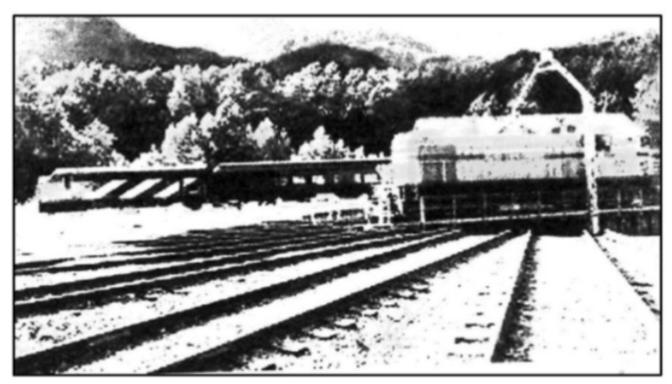
\includegraphics[width=0.8\columnwidth] {/storage/emulated/0/DCIM/Screenshots/figure1.jpg}
        \end {figure}                                                                                                  
\\ An exhibit in the museum depicted many rail lines on the track near the railway station. Let $L$ be the set of all rail lines on the railway track and $R$ be the relation on $L$ defined by
\begin {align*}
R=\cbrak{\brak{l_1,l_2}: l_1 \parallel l_2}
\end {align*}
On the basis of the above information, answer the following questions:

\begin {enumerate}
\item [(i)] Find whether the relation $R$ is symmetric or not.
\item [(ii)] Find whether the relation $R$ is transitive or not.
\item [(iii)] If one of the rail lines on the  railway track is represented by the equation $y=3x+2$, then find the set of rail lines in $R$ related to it.
\end {enumerate}
\item [(b)] Let $S$ be the relation defined by
        S=$\cbrak{\brak{l_1, l_2}:l_1 \perp l_2}$ check whether the relation $S$ is symmetric and transitive.
\end {enumerate}
\end {enumerate}

\section {Calculus}
\begin {enumerate}
\item A rectangular visiting card is to contain $24\,sq.cm$ of printed matter. The margins at the top and bottom of the card are to be $1\,cm$ and the margins on the left and right are to be $1 \frac{1}{2}cm$ as shown below :                                                              
	\begin {figure} [h!] 
	\centering  
	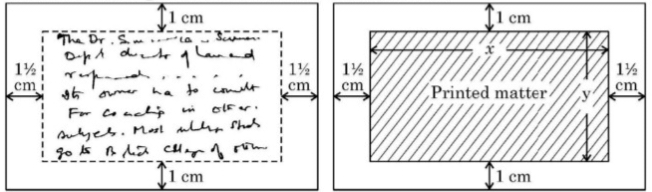
\includegraphics[width=0.8\columnwidth] {/storage/emulated/0/DCIM/Screenshots/figure2.jpg}          \end {figure}                                                                             \\On the basis of the above information, answer the following questons:
        \begin {enumerate}
\item [(i)] Write the expression for the area of the visiting card in terms of x.
\item [(ii)] Obtain the dimensions of the card of minimum area.
        \end {enumerate}
\end {enumerate}

\section {Optimization}
\begin {enumerate}
\item Solve the following L.P.P. graphically :\\Maximize $Z=60x+40y$\\Subject to
        \begin {align*} 
	x+2y\leq12 \\
	2x+y\leq12 \\
	4x+5y\geq20\\  
	x,y\geq0
            \end {align*}
\end {enumerate}
\end {document}

